\documentclass[aspectratio=169]{beamer}

\usetheme{Berlin}
\usecolortheme{default}

\usepackage{fontspec}
\usepackage{booktabs}
\usepackage{amsmath}
\usepackage{graphicx}

\graphicspath{{../png/}}

\setbeamertemplate{caption}[numbered]
\setbeamertemplate{navigation symbols}{}

\title[Partition Assignment Trade-offs]{Trade-offs in Partition Assignment Policy intended for Distributed Deployment of Dynamic Graph Embedding Systems}
\author{Stefan Nožinić}
\institute{Seminar 3}
\date{\today}

\begin{document}

\begin{frame}
  \titlepage
\end{frame}

\begin{frame}{Outline}
  \tableofcontents
\end{frame}

% ============================================================
\section{Motivation}
% ============================================================

\begin{frame}{Motivation}
  \begin{itemize}
    \item Large, dynamic graphs must be embedded in a \textbf{distributed} setting: no single machine holds the whole graph.
    \item Vertices arrive \textbf{online} and must be assigned to a partition before their full neighborhood is known.
    \item Core trade-off:
    \begin{itemize}
      \item More partitions $\rightarrow$ better scalability, but can hurt embedding quality and balance.
      \item Replicating an uncertain vertex across partitions can recover quality, at extra computation cost.
    \end{itemize}
    \item This trade-off has not been systematically studied for dynamic graph embedding.
  \end{itemize}
\end{frame}

\begin{frame}{Problem Formulation}
  Given a dynamic graph with online vertex arrivals and a distributed dynnode2vec-style embedding model, how should partitions be assigned to new vertices to balance:
  \begin{itemize}
    \item embedding quality,
    \item partition balance,
    \item computational cost of maintaining the assignment?
  \end{itemize}
\end{frame}

% ============================================================
\section{Method}
% ============================================================

\begin{frame}{Buffered Event-Processing Pipeline}
  \begin{itemize}
    \item The graph is a stream of events $(t, u, v)$.
    \item Events are \textbf{buffered} before partition assignment, so decisions use a batch of neighbor information instead of a single edge.
    \item Once a buffer fills (\texttt{MAX\_BUFFER\_SIZE}):
    \begin{enumerate}
      \item assign partitions for the buffered vertices,
      \item update embeddings,
      \item clear the buffer.
    \end{enumerate}
    \item Each buffer $B_n$ applied to snapshot $G_n$ yields the next snapshot: $G_{n+1} = G_n \cup B_n$.
  \end{itemize}
\end{frame}

\begin{frame}{Partition Scoring Formula}
  Score of partition $p_i \in \mathcal{P}$ for a newly arriving vertex $v$:
  \[
    S(p_i, v) = N(p_i, v) - \mu \cdot \max\!\left(0,\; |p_i| - \alpha (1+\epsilon) \cdot \frac{1}{P}\sum_{p_j \in \mathcal{P}} |p_j|\right)
  \]
  \begin{itemize}
    \item $N(p_i, v)$ -- neighbors of $v$ already in $p_i$, within the current buffer
    \item $\mu$ -- capacity penalty coefficient
    \item $\alpha$ -- weight of the average partition size
    \item $\epsilon$ -- imbalance tolerance
    \item $|p_i|$ -- current size of partition $p_i$
  \end{itemize}
  Vertex $v$ is assigned to the top $RF$ scoring partitions (replication factor $RF$); ties are broken at random.
\end{frame}

% ============================================================
\section{Experimental Setup}
% ============================================================

\begin{frame}{Datasets}
  \footnotesize
  \begin{tabular}{lrrrrrr}
    \toprule
    Dataset & Nodes & Edges & Avg. deg. & Avg. clust. & Density & Modularity \\
    \midrule
    CITESEER   & 3264  & 4536   & 2.78  & 0.145 & 0.00090 & 0.72 \\
    DBLP       & 17716 & 52867  & 5.97  & 0.134 & 0.00034 & 0.58 \\
    AstroPh    & 18772 & 198110 & 21.11 & 0.631 & 0.00112 & 0.33 \\
    AS-Oregon  & 11806 & 38781  & 6.57  & 0.399 & 0.00056 & 0.57 \\
    Enron      & 36692 & 183831 & 10.02 & 0.497 & 0.00027 & 0.36 \\
    \bottomrule
  \end{tabular}
  \vspace{1em}

  Five real-world dynamic graphs, chosen to vary in size, density, and community structure.
\end{frame}

\begin{frame}{Static Baseline and Hyperparameters}
  \begin{columns}
    \begin{column}{0.48\textwidth}
      \centering
      \small Static node2vec F1 (unpartitioned)
      \begin{tabular}{lr}
        \toprule
        Dataset & F1 \\
        \midrule
        CITESEER   & 34.82\% \\
        DBLP       & 60.3\%  \\
        AstroPh    & 70.41\% \\
        AS-Oregon  & 31.26\% \\
        Enron      & 20.42\% \\
        \bottomrule
      \end{tabular}
    \end{column}
    \begin{column}{0.48\textwidth}
      \centering
      \small Partitioning hyperparameters
      \begin{tabular}{lr}
        \toprule
        Hyperparameter & Value \\
        \midrule
        Buffer size & 1000 \\
        $\mu$       & 1 \\
        $\alpha$    & 1 \\
        $\epsilon$  & 0.1 \\
        $P$         & $\{1,2,4,8\}$ \\
        $RF$        & 1 \\
        \bottomrule
      \end{tabular}
    \end{column}
  \end{columns}
  \vspace{1em}
  These static F1 scores are a rough upper bound: a partitioned, incremental system generally should not exceed them.
\end{frame}

% ============================================================
\section{Results}
% ============================================================

\begin{frame}{F1 Reconstruction Score vs.\ Partition Count}
  \small
  \begin{tabular}{lrrrr}
    \toprule
    Dataset & $P=1$ & $P=2$ & $P=4$ & $P=8$ \\
    \midrule
    CITESEER   & 47.57\% & 45.81\% & 48.06\% & 54.81\% \\
    DBLP       & 50.91\% & 54.11\% & 54.51\% & 49.87\% \\
    AstroPh    & 57.70\% & 54.67\% & 50.95\% & 45.94\% \\
    AS-Oregon  & 26.17\% & 24.88\% & 24.30\% & 21.45\% \\
    Enron      & 18.03\% & 24.84\% & 27.44\% & 32.36\% \\
    \bottomrule
  \end{tabular}
  \vspace{1em}
  \begin{itemize}
    \item AstroPh, AS-Oregon: quality \textbf{degrades} as $P$ grows.
    \item CITESEER, DBLP, Enron: quality \textbf{stable or improves} over most of the range.
  \end{itemize}
\end{frame}

\begin{frame}{Edge Cut and Balance vs.\ Partition Count}
  \begin{columns}
    \begin{column}{0.48\textwidth}
      \centering
      \small Edge cut (\%)
      \begin{tabular}{lrrrr}
        \toprule
        Dataset & $P{=}1$ & $P{=}2$ & $P{=}4$ & $P{=}8$ \\
        \midrule
        CITESEER  & 0 & 23 & 39 & 48 \\
        DBLP      & 0 & 32 & 50 & 59 \\
        AstroPh   & 0 & 35 & 56 & 65 \\
        AS-Oregon & 0 & 30.4 & 53.8 & 71.6 \\
        Enron     & 0 & 33.1 & 49.2 & 62.0 \\
        \bottomrule
      \end{tabular}
    \end{column}
    \begin{column}{0.48\textwidth}
      \centering
      \small Balance ($B{=}1$ is ideal)
      \begin{tabular}{lrrrr}
        \toprule
        Dataset & $P{=}1$ & $P{=}2$ & $P{=}4$ & $P{=}8$ \\
        \midrule
        CITESEER  & 1 & 1.31 & 1.63 & 1.75 \\
        DBLP      & 1 & 1.10 & 1.20 & 1.31 \\
        AstroPh   & 1 & 1.08 & 1.11 & 1.26 \\
        AS-Oregon & 1 & 1.21 & 1.26 & 1.27 \\
        Enron     & 1 & 1.09 & 1.08 & 1.25 \\
        \bottomrule
      \end{tabular}
    \end{column}
  \end{columns}
  \vspace{1em}
  \small Edge cut grows monotonically with $P$ on every dataset; balance stays near 1 for all datasets except CITESEER.
\end{frame}

\begin{frame}{Why the Dataset-Dependent Split?}
  \begin{itemize}
    \item Signed F1 change $P{=}1 \to P{=}8$ correlates most strongly with graph \textbf{density} (Spearman $\rho \approx -0.7$).
    \item Weaker correlation with modularity ($\rho \approx +0.4$) and clustering coefficient ($\rho \approx -0.3$).
    \item No single property cleanly separates the two groups:
    \begin{itemize}
      \item CITESEER (improves) is denser than AS-Oregon (degrades).
      \item Enron has the lowest density and modularity among the stable group, yet the largest improvement.
    \end{itemize}
    \item Density is the closest available proxy, but not a complete explanation.
  \end{itemize}
\end{frame}

\begin{frame}{Buffer Size Sensitivity}
  \centering
  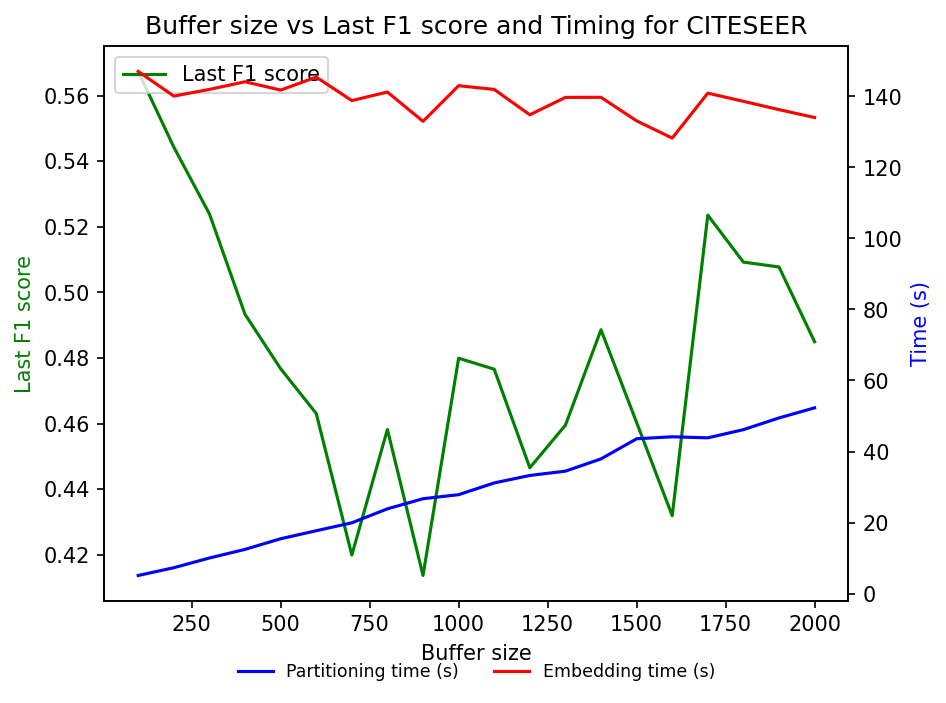
\includegraphics[width=0.47\textwidth]{citeseer-buffer-timing.png}
  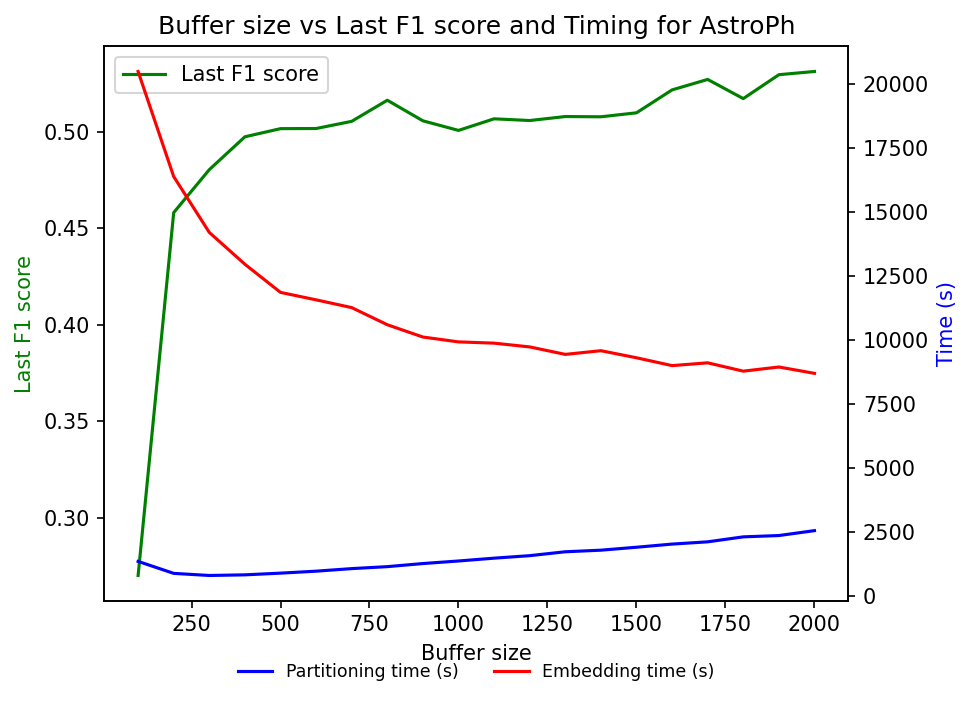
\includegraphics[width=0.47\textwidth]{astroph-buffer-timing.png}
  \begin{itemize}
    \footnotesize
    \item AstroPh: larger buffers clearly help (F1 $\approx 0.27 \to 0.53$).
    \item CITESEER: larger buffers do \emph{not} help; best F1 at the smallest buffer size.
    \item Partitioning time grows with buffer size but stays smaller than embedding time throughout.
  \end{itemize}
\end{frame}

\begin{frame}{Capacity Penalty ($\mu$) Sensitivity}
  \centering
  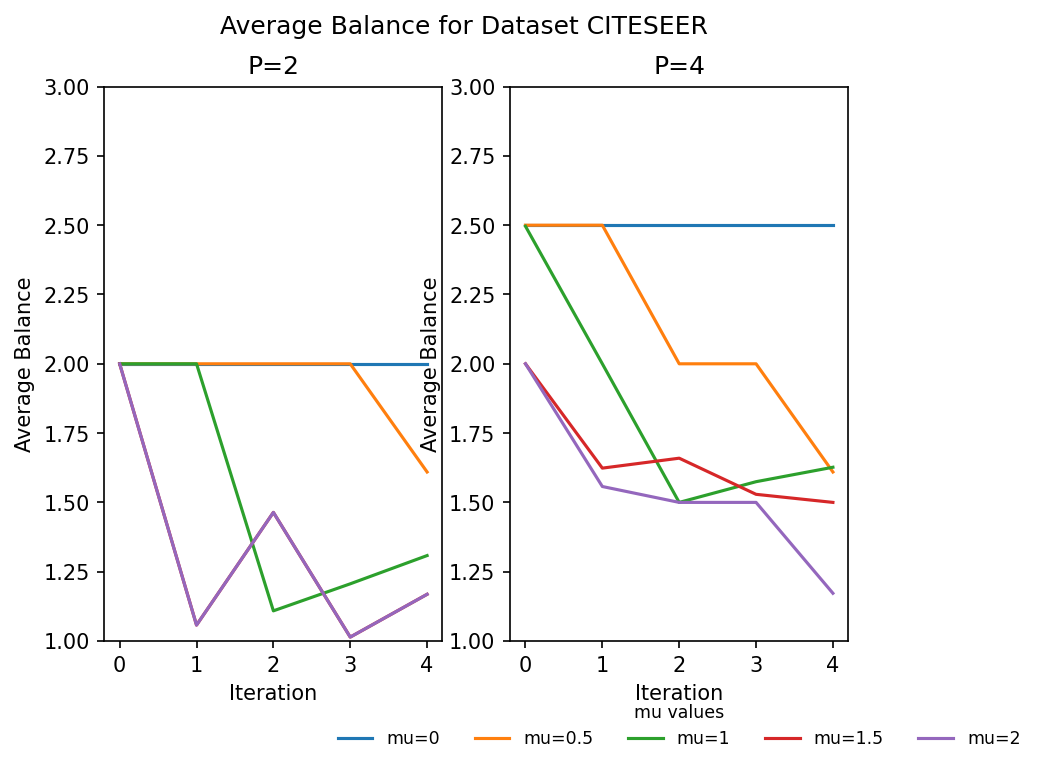
\includegraphics[width=0.40\textwidth]{citeseer-balance-mu.png}
  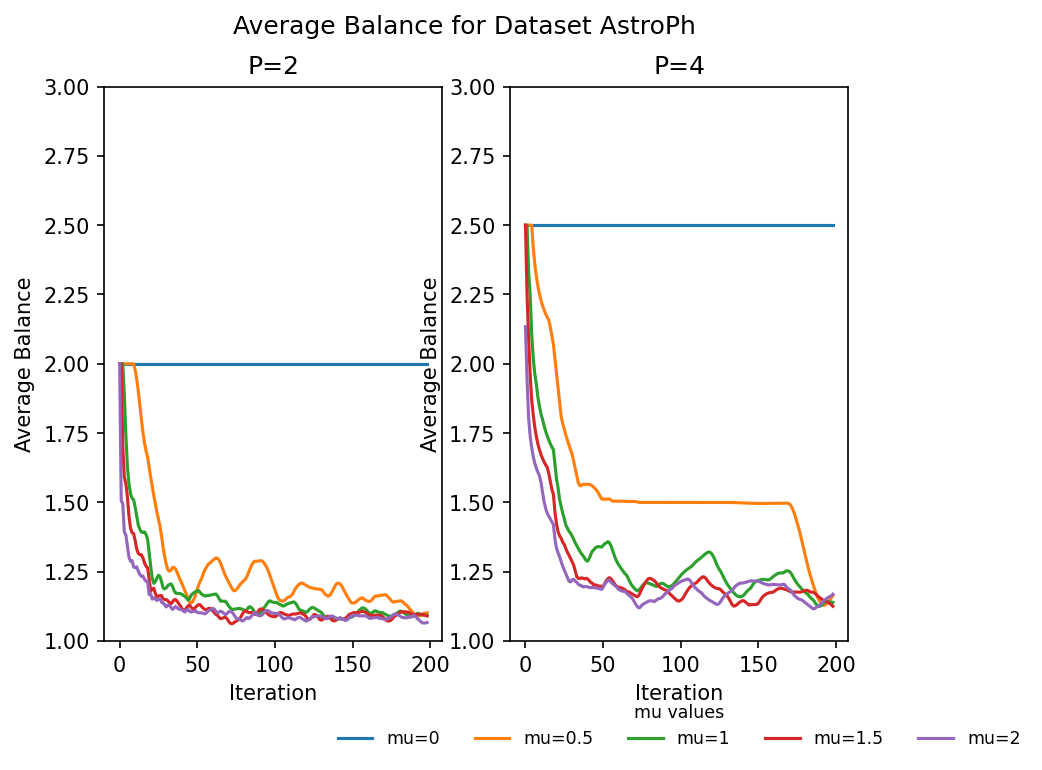
\includegraphics[width=0.40\textwidth]{astroph-balance-mu.png}
  \vspace{-2mm}
  \begin{itemize}
    \footnotesize
    \item $\mu=0$ collapses all vertices into one partition (worst balance: 2.00 / 2.50 at $P{=}2/4$).
    \item Increasing $\mu$ from 0 to 1 gives the largest balance improvement; returns diminish beyond $\mu \approx 1$--$1.5$.
    \item Better balance is bought at a real F1 cost (e.g.\ AstroPh $P{=}8$: 57.00\%~$\to$~33.93\% at $\mu{=}0.5$).
  \end{itemize}
\end{frame}

\begin{frame}{Random Partitioner Baseline}
  \small
  \begin{columns}
    \begin{column}{0.48\textwidth}
      \centering CITESEER
      \begin{tabular}{lrrr}
        \toprule
        $P$ & F1 & Edge cut & Balance \\
        \midrule
        2 & 0.03\% & 50.0\% & 1.02 \\
        4 & 0.03\% & 70.9\% & 1.32 \\
        8 & 0.04\% & 81.6\% & 1.61 \\
        \bottomrule
      \end{tabular}
    \end{column}
    \begin{column}{0.48\textwidth}
      \centering AstroPh
      \begin{tabular}{lrrr}
        \toprule
        $P$ & F1 & Edge cut & Balance \\
        \midrule
        2 & 0.04\% & 50.0\% & 1.00 \\
        4 & 0.03\% & 70.9\% & 1.31 \\
        8 & 0.02\% & 81.4\% & 1.60 \\
        \bottomrule
      \end{tabular}
    \end{column}
  \end{columns}
  \vspace{1em}
  Random assignment collapses F1 to $\approx 0$: the neighbor partitioner's quality genuinely comes from preserving neighborhood locality, not from the embedding algorithm alone.
\end{frame}

\begin{frame}{Effect of Replication Factor}
  \begin{itemize}
    \item Replication lets a vertex be embedded in more than one partition; the final embedding is the average of the per-partition embeddings.
    \item Preliminary sweep on CITESEER, $P=4$, buffer size 1000, $\mu=1$:
    \begin{itemize}
      \item $RF=1$: F1 $= 44.35\%$
      \item $RF=3$: F1 $= 69\%$
    \end{itemize}
    \item Large recovery of embedding quality lost to early, uncertain assignment -- at the cost of up to $RF\times$ the embedding computation per vertex.
    \item Single-configuration result: promising, but not yet systematically validated.
  \end{itemize}
\end{frame}

\begin{frame}{Temporal Evolution: Repartitioning Rate}
  \centering
  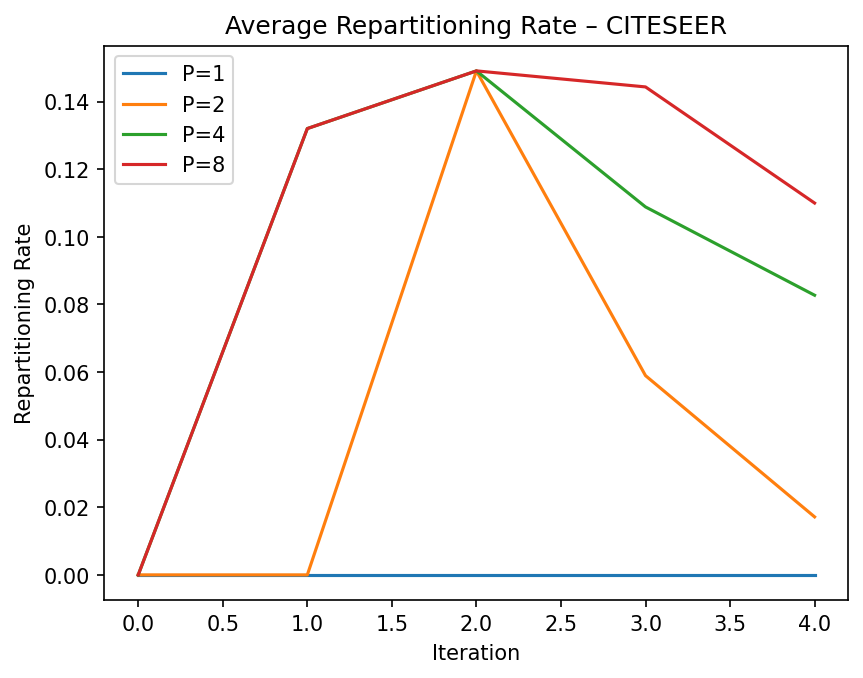
\includegraphics[width=0.24\textwidth]{citeseer-repartitions.png}
  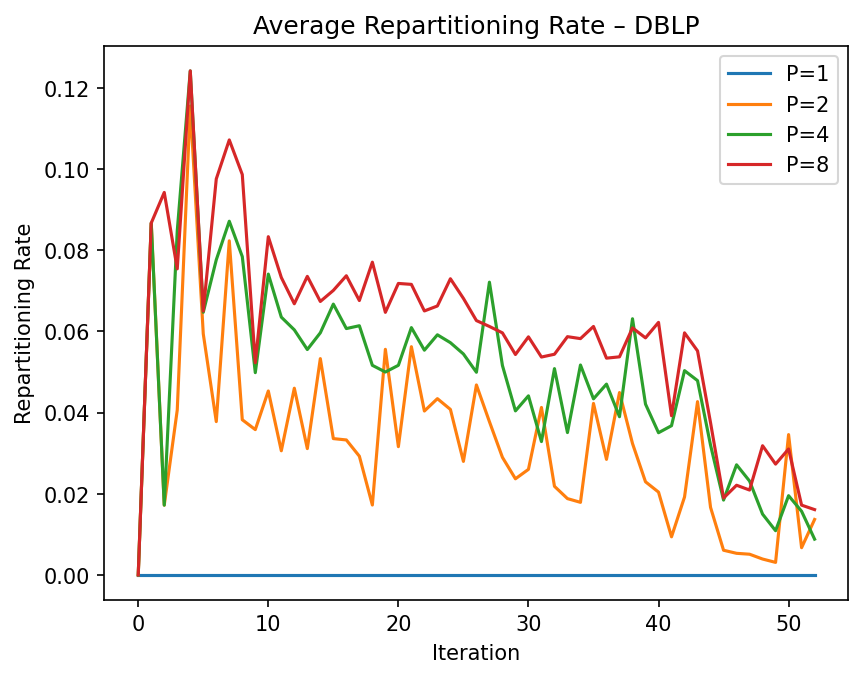
\includegraphics[width=0.24\textwidth]{dblp-repartitions.png}
  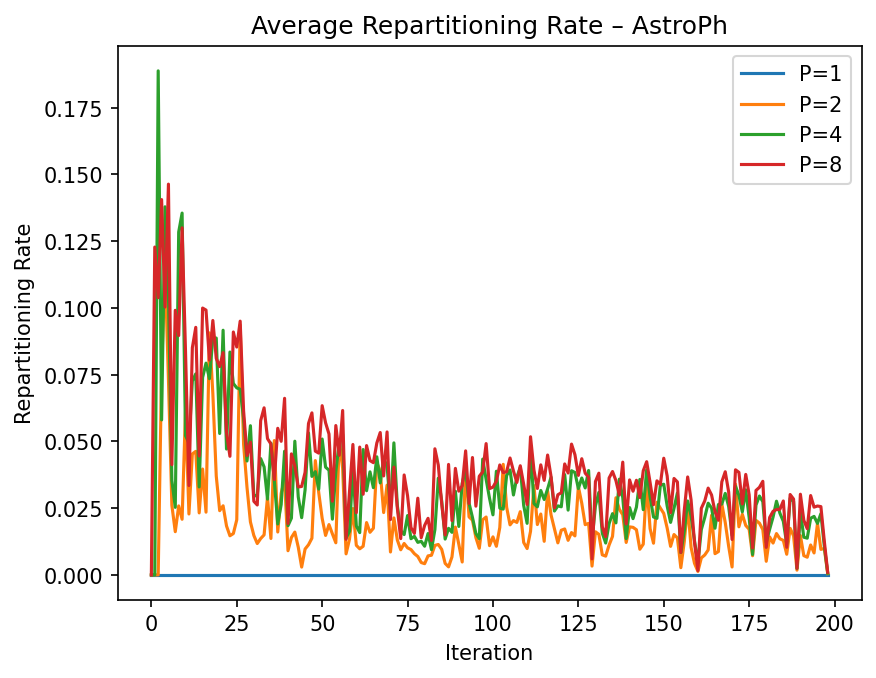
\includegraphics[width=0.24\textwidth]{astroph-repartitions.png}\\[0.5mm]
  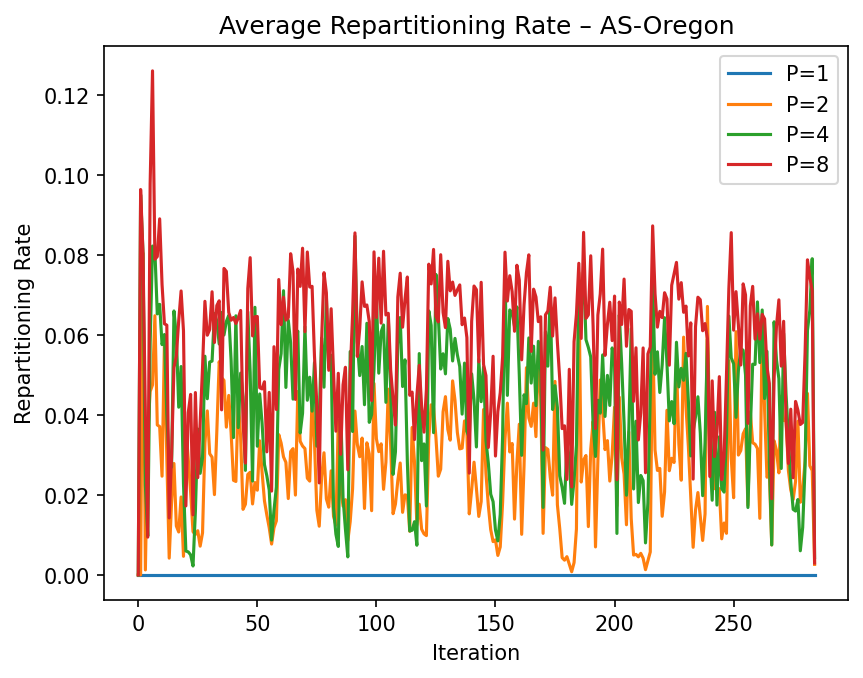
\includegraphics[width=0.24\textwidth]{as-oregon-repartitions.png}
  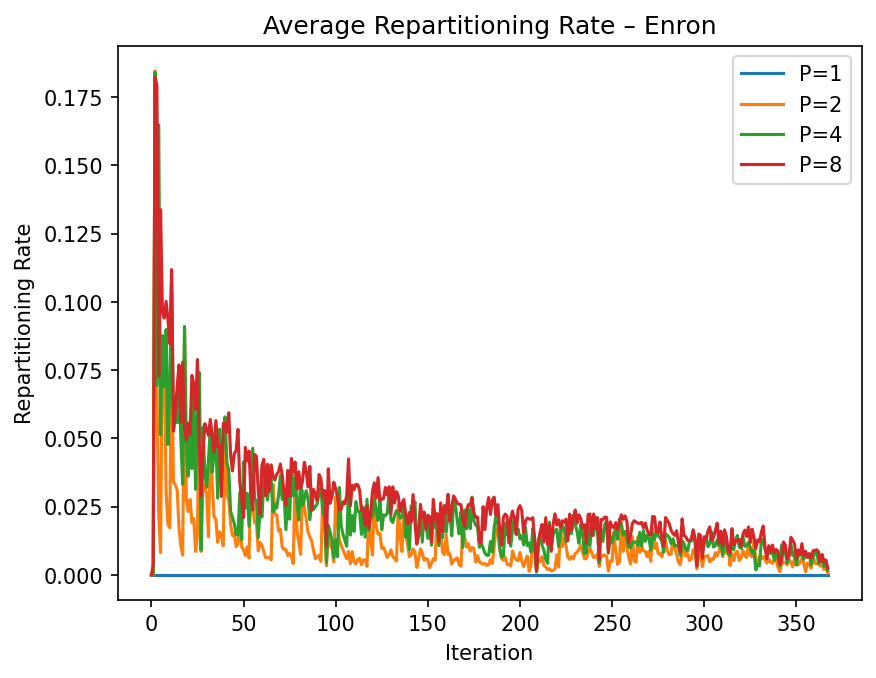
\includegraphics[width=0.24\textwidth]{enron-repartitions.png}
  \vspace{-2mm}

  \footnotesize Repartitioning rate decays rapidly after an initial warm-up and stays below 20\% across all datasets and partition counts -- assignments stabilize quickly.
\end{frame}

% ============================================================
\section{Conclusion}
% ============================================================

\begin{frame}{Conclusion}
  \begin{itemize}
    \item Impact of partitioning on embedding quality is \textbf{dataset-dependent}: AstroPh and AS-Oregon degrade; CITESEER, DBLP, and Enron are stable or improve, with DBLP reversing sharply at $P=8$.
    \item Graph density correlates most closely with this split, but does not fully explain it.
    \item The neighbor-based partitioner keeps balance close to ideal (except CITESEER) and repartitioning rate low, without explicit rebalancing.
    \item Partitioning time stays consistently smaller than embedding time.
    \item Replication factor is a promising, preliminary lever for recovering quality lost to early assignment.
  \end{itemize}
\end{frame}

\begin{frame}{Future Work}
  \begin{itemize}
    \item Direct comparison of delayed vs.\ immediate assignment, measuring latency alongside quality.
    \item Systematic replication factor sweep across datasets and partition counts.
    \item Evaluate embeddings on downstream tasks (link prediction, node classification), beyond reconstruction F1.
  \end{itemize}
\end{frame}

\begin{frame}
  \centering
  \Large Thank you!
\end{frame}

\end{document}
